\chapter{Deep Learning}

Not only in Computer Vision, such as object detection but also in natural language processing or speech recognition, and even human-level video game play deep neural networks are used to solve domain specific tasks. In this chapter it shall be explained how those networks function by going into details with a feed-forward neural network. Furthermore a glimpse is taken about tricks of the trade such as batch normalization and initialization.


\section{Feed-Forward Neural Networks}
A feed-forward neural network consist of one input layer, H hidden layers and one output layer. Each layer consist of units (or neurons) where each unit of a given layer is fully- connected to every unit of the previous layer. The graphical representation can be described mathematically as a combination of matrix multiplication and activation functions. The activation function models when an artificial neuron fires and is usually a non-linearity. In theory, it is this non-linear activation function, which allows the network to learn any function approximation. Each unit in a hidden layer can be mathematically described by:

\begin{equation}
	y_{j} = f(z_{j})
\end{equation}

\begin{equation}
z_{j} = \sum w_{ij}*x_{i} + b_{j}
\end{equation}

\begin{figure}[H]
	\centering
	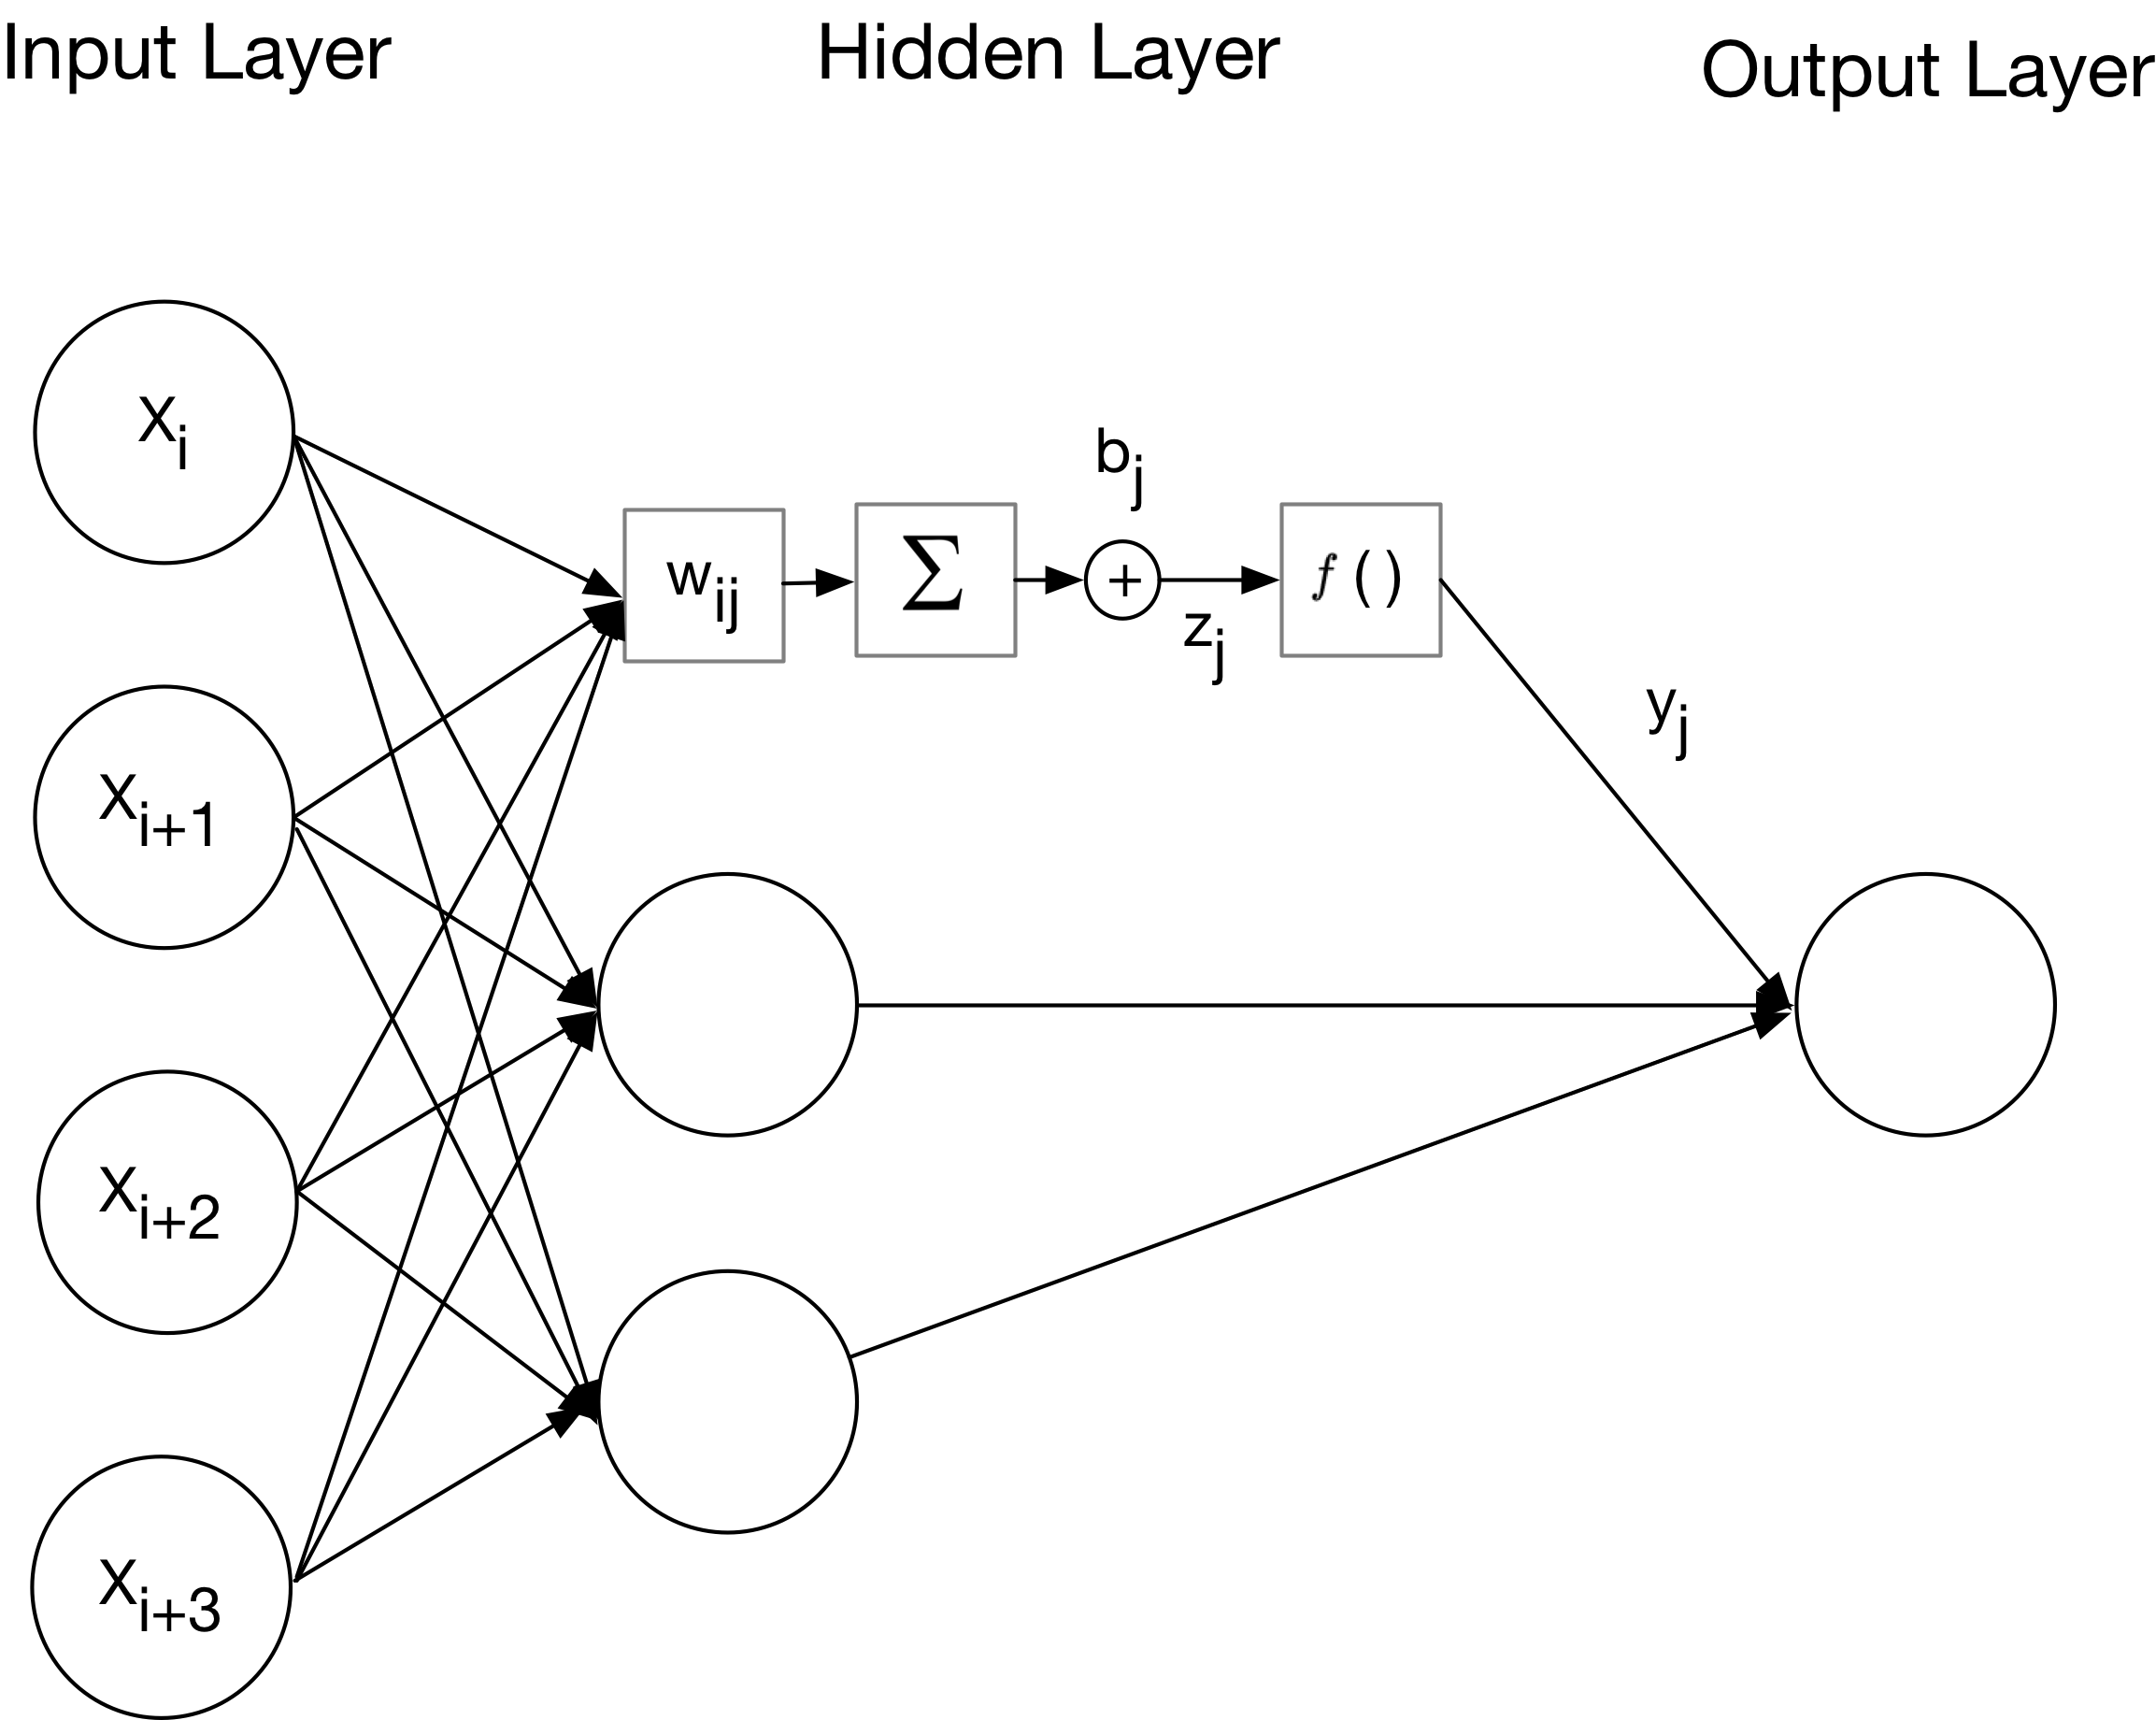
\includegraphics[width=0.8\linewidth]{bilder/grundlagen/fast-forward.png}
	\caption{Schematic view of a FCN. Schematic of a simple two layer fully connected neural network (FCN)} source: Own illustration
	\label{fig:FCN}
\end{figure}



Where \( y_{i} \) is the output of the unit from the current layer. The output is transformed with a non-linear activation function. \(z\) is called the preactivation and \(w\) denotes the edge weights. \( x_{i} \) is the output of a unit from the previous layer. At every layer first the total input \(z\) is computed, \(z\) is the weighted sum of the outputs from the layer before. After that a non linear function \( f(\cdot) \)is applied to \(z\) in order to get the output \( y_{j} \) of the unit. 

All differential functions can be used as a activation function of a neural network. Most common activation functions are sigmoid,  \(f(z) = \frac{1}{exp(-z)}\), the hyperbolic tangent, \(f(z) = \frac{exp(z)-exp(-z)}{exp(z)+exp(-z)}\) or the rectifier linear unit (ReLU) \(f(z) = max(0; z)\). ReLu will be used for all future examples.


\begin{figure}[H]
	\centering
	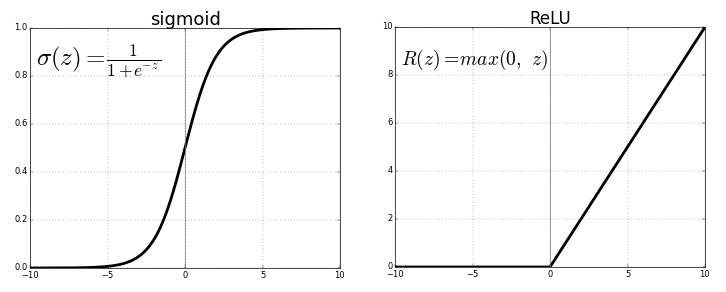
\includegraphics[width=0.8\linewidth]{bilder/grundlagen/sigmoid.png}
	\caption{Sigmoid And ReLu Activation Function} source:\cite{Component}
	\label{fig:COMPONENT}
\end{figure}


\subsection{Backpropagation}

To train a neural network two things need to be done. First a forward pass, second an error backpropagation. Given a certain input, a forward pass calculates the output of each unit. A predefined cost function \(E\) then compares the resulting outputs \(y_{out}\) with the correct answer and determines the error. A common cost function for example is 
squared error loss.

\begin{equation}
E=\sum\dfrac{1}{2} (target-y_{out}^2) 
\end{equation}
	
Given this error it is now possible to check how weights need to be adjusted in order to bring the \(E\) to a minimum. By applying chain rule of derivatives. 
\begin{equation}
\frac{\partial z}{\partial x} = \frac{\partial z}{\partial y} \frac{\partial y}{\partial x}
\end{equation}

Taking the Error in consideration the algebra looks like this:

\begin{equation}
\Delta_{W}E =
\frac{\partial E}{\partial W_{l}} =
\frac{\partial E}{\partial y_{out}}
\frac{\partial y_{out}}{\partial z_{out}}
\frac{\partial z_{out}}{\partial y_{n-1}}
\frac{\partial y_{n-1}}{\partial z_{n-1}}
\end{equation}

Using the calculated gradient $\Delta_{W}E(y_{out}) $ it is now possible to determine next update for the weights matrix by a gradient descent update:

\begin{equation}
W_{l}^{t+1}=
W_{l}^{t}-\eta\Delta_{W_{l}^{t}}E(y_{yout)}
\end{equation}

Where \(W^{t}\), \(W^{t+1}\) are the current weights and the weight matrix for the updated weights. \(\eta\) is the learning rate.

\subsection{Weight Update}
It requires a lot of computation time to calculate the gradient from whole dataset. Mini-batches can be used to calculate the gradient only based on a few sampled data points. Using this analytic gradient a parameter update is performed. There are several ways to do this update. But the most common way is Stochastic gradient descent (SGD). 
Parameters are simply changed along the negative gradient direction in order to minimize the error.


\subsection{Initialization}
To train a neural network initial weights need to be set. The most common way is a random initialization were every value is randomly set for example from a Gaussian.

\subsection{Batch normalization}
To avoid too big values or too small values in data a normalization is performed.

\begin{equation}
x \Rightarrow \hat{x} = \dfrac{x-\mu}{\sigma} \Rightarrow x_{norm} = \gamma \hat{x} + \beta
\end{equation}

\(\mu\) and \(\sigma\) are mean standard deviation of the dataset. 
\(gamma\)\ and \(\sigma\) scale and shift the parameters. Batch normalization accelerates training time and makes a deep neural network less sensitive to initialization issues.

\section{Classification}
A really common problem for neural networks is the classification of images, or more general the classification of data into a specific category. The best performing neural network architecture for classifying images are convolutional neural networks. All convolutional neural networks consist of convolutional layers followed by pooling layers and some fully connected layers.

\subsection{Convolutional layer}
In the convolutional layer several kernels are applied to extract spacial related features. Each output from the the convolutional layer is called a feature-map. Each feature-map was created by a different convolutional kernel of the layer. 

\begin{figure}[H]
	\centering
	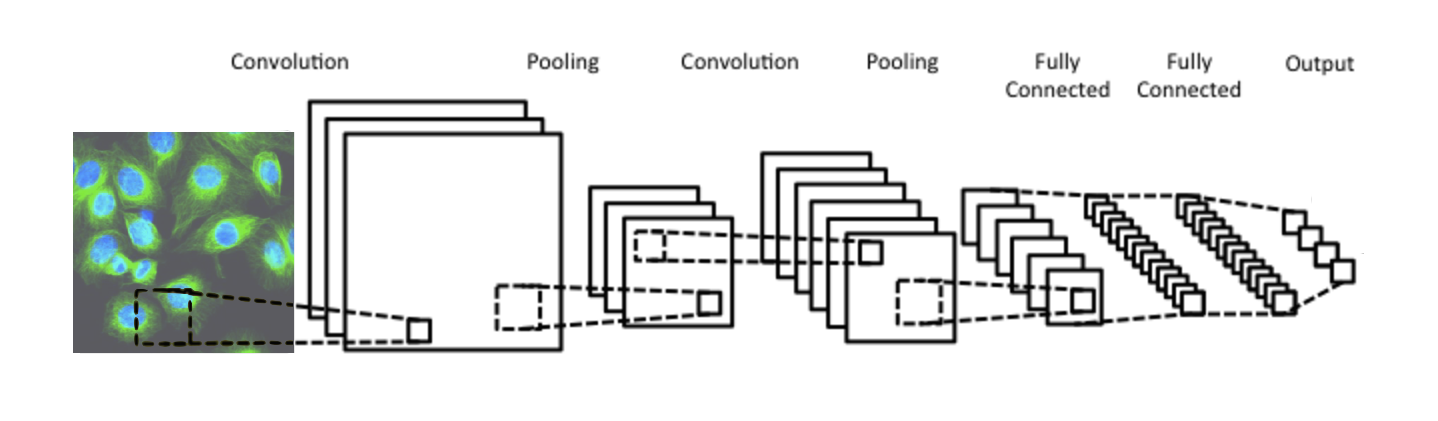
\includegraphics[width=\linewidth]{bilder/grundlagen/convolution.png}
	\caption{Schematic view of a FCN. Schematic of a simple two layer fully connected neural network (FCN)} source:\cite{Component}
	\label{fig:COMPONENT}
\end{figure}

\subsection{Pooling layer}
After features were extracted into feature maps the pooling layer reduces the size of the feature maps and makes the computation tractable. A very simple implementation of a pooling layer is the max-pooling layer, which uses a sliding windows over the input and selects the maximum of each window.

\begin{figure}[H]
	\centering
	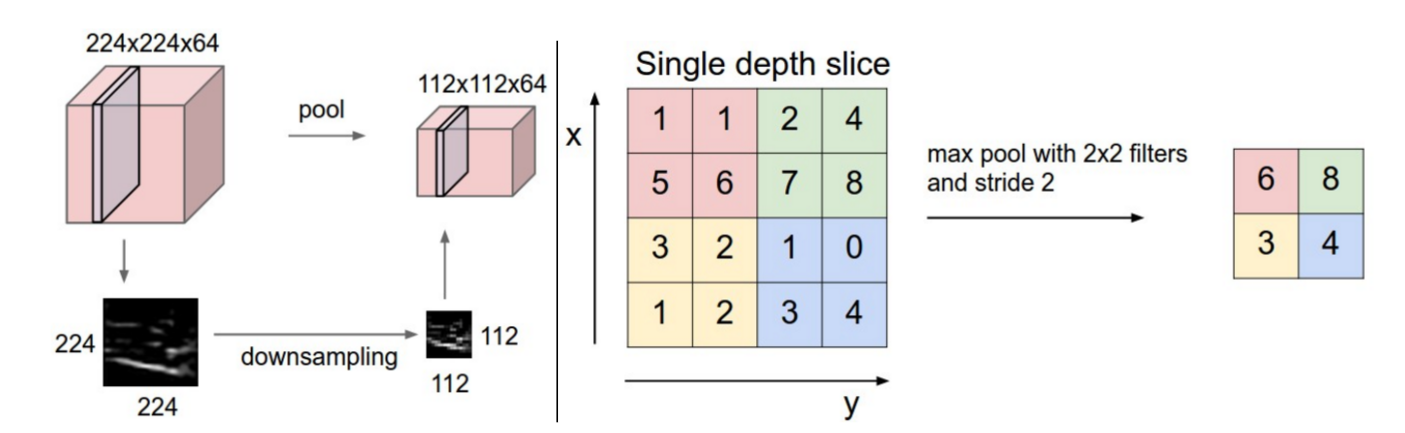
\includegraphics[width=\linewidth]{bilder/grundlagen/pooling.png}
	\caption{Schematic view of a FCN. Schematic of a simple two layer fully connected neural network (FCN)} source:\cite{Component}
	\label{fig:COMPONENT}
\end{figure}

\subsection{Data augmentation}
Convolutional neural networks need a lot of data to generate suffice output. If not enough data can be provided the data can be artificially augmented by using different approaches. Pictures can be turned or flipped, cropped, blurred or even resized. This makes it possible to generate a lot of data which can be used to further improve training.

\begin{figure}[H]
	\centering
	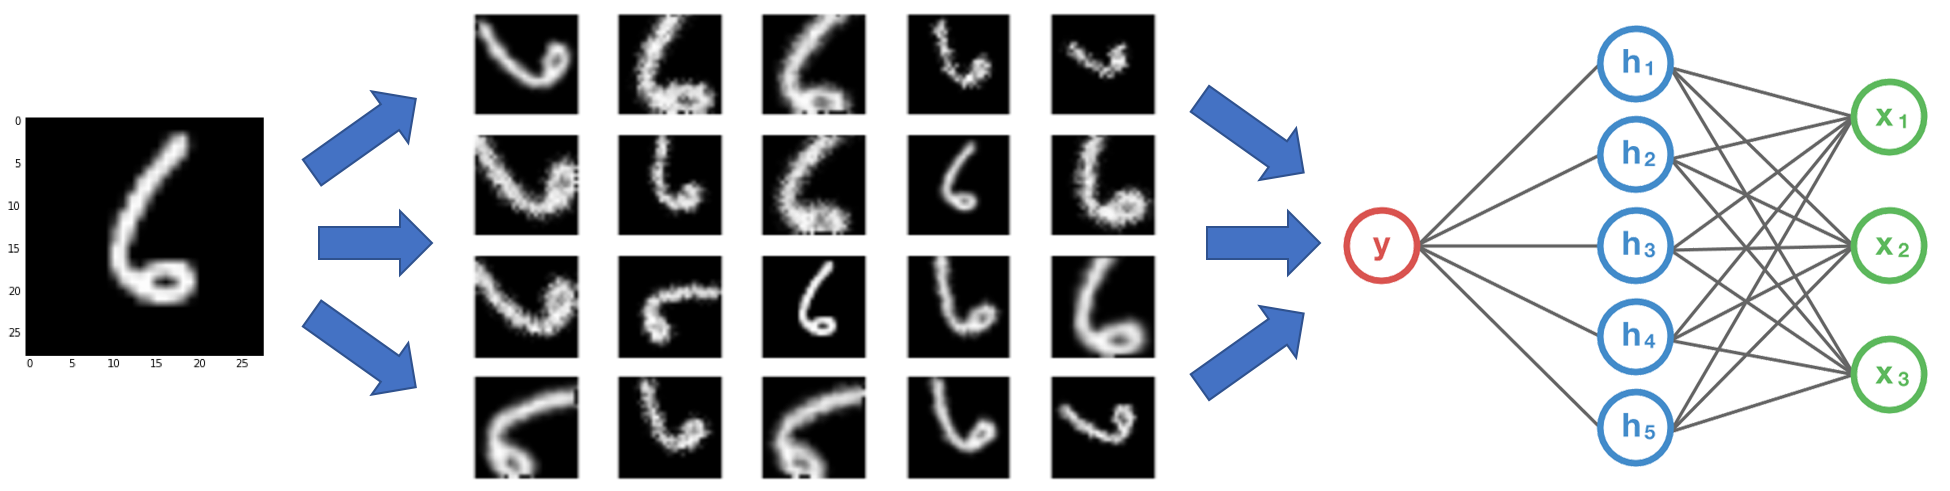
\includegraphics[width=\linewidth]{bilder/deep_learning/data_aug_basic.png}
	\caption{Data Augmentation} source:\cite{Component}
	\label{fig:COMPONENT}
\end{figure}

